\documentclass[11pt, a4paper]{book}
\usepackage[bahasa]{babel}
\usepackage[utf8]{inputenc}
\usepackage{graphicx}
\usepackage{hyperref}
\usepackage{quoting}
\usepackage{listings}
\usepackage{xcolor}
\usepackage{tabularx}
\usepackage{adjustbox}
\usepackage{tikz}
\usepackage{float}
\usepackage{minted}
\usepackage{caption}
\usetikzlibrary{shapes,arrows,positioning}
\usepackage{amsmath}
\usepackage{fancyhdr}

% Layout packages
\usepackage[top=2.5cm, bottom=2.5cm, left=3cm, right=2.5cm]{geometry}
\usepackage{setspace}
\onehalfspacing

% Modern heading styles
\usepackage{titlesec}
\titleformat{\chapter}[hang]
{\normalfont\LARGE\bfseries}{\thechapter.}{1em}{}
\titlespacing*{\chapter}{0pt}{-20pt}{40pt}

\titleformat{\section}
{\normalfont\Large\bfseries}{\thesection}{1em}{}
\titlespacing*{\section}{0pt}{3.5ex plus 1ex minus .2ex}{2.3ex plus .2ex}

\setminted{
	breaklines=true,
	breakanywhere=true,
	fontsize=\scriptsize,
	breakafter=/ ,
	breakbefore=. ,
	breaksymbolleft=,
	breakaftersymbolpre=,
	breakaftersymbolpost=
}

\definecolor{codegreen}{rgb}{0,0.6,0}
\definecolor{codegray}{rgb}{0.5,0.5,0.5}
\definecolor{codepurple}{rgb}{0.58,0,0.82}
\definecolor{backcolour}{rgb}{0.95,0.95,0.92}
\definecolor{LightGray}{gray}{0.95}

\lstdefinestyle{mystyle}{
	backgroundcolor=\color{backcolour},   
	commentstyle=\color{codegreen},
	keywordstyle=\color{magenta},
	numberstyle=\tiny\color{codegray},
	stringstyle=\color{codepurple},
	basicstyle=\ttfamily\footnotesize,
	breakatwhitespace=false,         
	breaklines=true,                 
	captionpos=b,                    
	keepspaces=true,                 
	numbers=left,                    
	numbersep=5pt,                  
	showspaces=false,                
	showstringspaces=false,
	showtabs=false,                  
	tabsize=2
}

% Configure listings
\lstset{
	basicstyle=\ttfamily\small,
	breaklines=true,
	breakindent=0pt,
	breakatwhitespace=true,
	postbreak=\mbox{\textcolor{gray}{$\hookrightarrow$}\space},
	columns=flexible,
	frame=single,
	keepspaces=true,
	showstringspaces=false,
	tabsize=2,
	linewidth=\textwidth,
	xleftmargin=\parindent,
	xrightmargin=\parindent,
	belowskip=\medskipamount,
	aboveskip=\medskipamount,
	resetmargins=true,
	numbers=none,
	numberstyle=\tiny,
	commentstyle=\color{gray},
	keywordstyle=\color{black},
	stringstyle=\color{black},
	captionpos=b,
	flexiblecolumns=true,
	basewidth={0.5em,0.45em}
}

% Header and footer setup
\pagestyle{fancy}
\fancyhf{}
\renewcommand{\headrulewidth}{0.4pt}
\renewcommand{\footrulewidth}{0.4pt}
\fancyhead[L]{\leftmark}
\fancyhead[R]{\thepage}

% Hyperref setup
\hypersetup{
	colorlinks=true,
	linkcolor=black,
	filecolor=black,      
	urlcolor=black,
	pdftitle={Laporan Implementasi Sistem High-Availability dan Disaster Recovery Infrastruktur Odoo PT. Infrastruktur Digital Indonesia},
	pdfauthor={PT Allbest Solusi Sistem},
	pdfsubject={Laporan Implementasi Proyek},
	pdfkeywords={High-Availability, Disaster Recovery, Odoo, PostgreSQL, PeerDB, Replikasi, Server, Backup, PT Ideanet, PT Allbest}
}

\title{Memahami Distributed Caching: Rahasia Dibalik Aplikasi Cepat}
\author{chmdznr}
\date{}

\begin{document}
	
	\maketitle
	
	\tableofcontents
	\listoffigures
	\clearpage
	
	\chapter{Dasar-dasar Caching}
	\label{chap:dasar-caching}
	
	\section{Konsep Umum Caching}
	\label{sec:konsep-umum}
	
	\begin{itemize}
		\item \textbf{Definisi}: Caching adalah teknik penyimpanan data sementara di lokasi yang mudah diakses untuk mengurangi waktu respons
		
		\item \textbf{Analog}:
		\begin{itemize}
			\item Meja kerja vs. gudang arsip
			\item Gerai cepat di minimarket
		\end{itemize}
		
		\item \textbf{Terminologi Penting}:
		\begin{itemize}
			\item \textbf{Cache Hit}: Data ditemukan di cache
			\item \textbf{Cache Miss}: Data tidak ditemukan di cache
			\item \textbf{TTL (Time-to-Live)}: Waktu kedaluwarsa data cache
			\item \textbf{Invalidasi}: Proses penghapusan data cache sebelum TTL
		\end{itemize}
	\end{itemize}
	
	\section{Perbandingan dengan Query Database Tradisional}
	\label{sec:perbandingan}
	
	\begin{table}[H]
		\centering
		\caption{Perbandingan Karakteristik Caching vs Database}
		\label{tab:perbandingan}
		\begin{tabularx}{\textwidth}{|l|X|X|}
			\hline
			\textbf{Parameter} & \textbf{Caching} & \textbf{Database} \\ \hline
			Latensi & Milidetik (ms) & 10-100x lebih tinggi \\ \hline
			Throughput & Ribuan operasi/detik & Terbatas I/O disk \\ \hline
			Pola Akses & Data panas (hot data) & Data lengkap \\ \hline
			Biaya & Memory-intensive & Storage-intensive \\ \hline
		\end{tabularx}
	\end{table}
	
	\subsection{Alur Kerja Dasar}
	\label{subsec:alur-kerja}
	
	\begin{figure}[H]
		\centering
		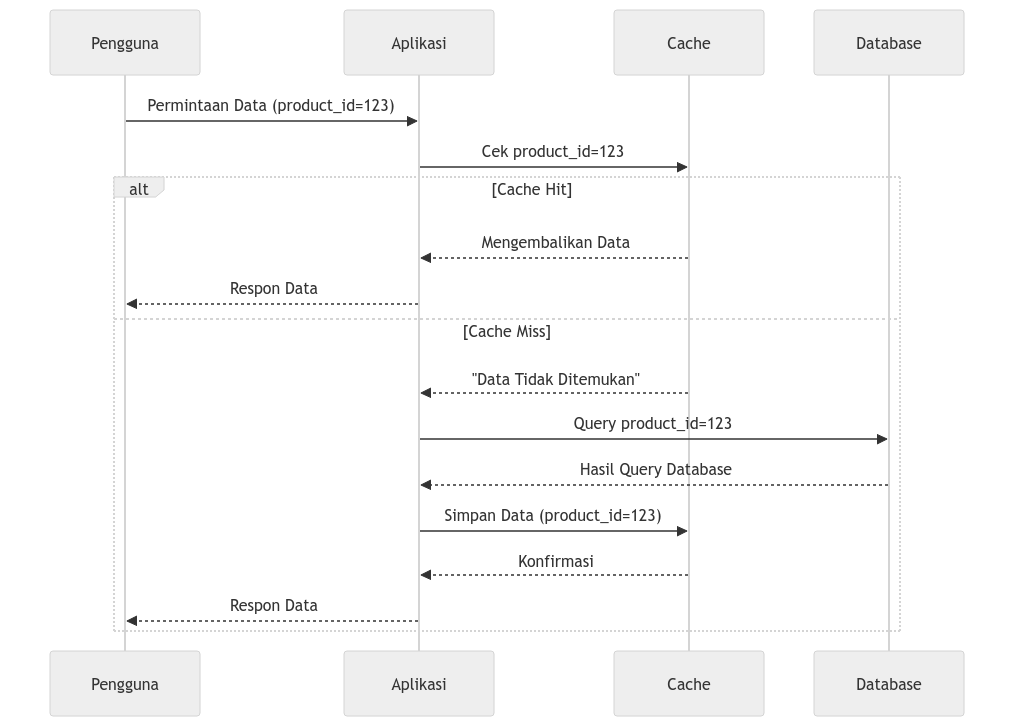
\includegraphics[width=0.9\textwidth]{images/workflow-cache.png}
		\caption{Alur kerja sistem dengan caching}
		\label{fig:workflow}
	\end{figure}
	
	\begin{enumerate}
		\item Aplikasi menerima permintaan data
		\item Cek cache pertama:
		\begin{itemize}
			\item Jika \textbf{hit}: Langsung kembalikan data
			\item Jika \textbf{miss}: Ambil dari database
		\end{itemize}
		\item Simpan hasil query database ke cache
		\item Kembalikan data ke pengguna
	\end{enumerate}
	
	\section{Manfaat dan Tantangan}
	\label{sec:manfaat-tantangan}
	
	\subsection{Manfaat Utama}
	\label{subsec:manfaat}
	
	\begin{itemize}
		\item Mengurangi latensi hingga 90\% 
		\item Menurunkan beban database
		\item Meningkatkan throughput sistem
		\item Menghemat biaya infrastruktur
	\end{itemize}
	
	\subsection{Tantangan Umum}
	\label{subsec:tantangan}
	
	\begin{itemize}
		\item \textbf{Data Stale}: Risiko data tidak update
		\item \textbf{Cache Stampede}: Lonjakan permintaan saat cache expired
		\item \textbf{Memory Management}: Alokasi memori yang efisien
		\item \textbf{Complexity}: Penambahan layer infrastruktur
	\end{itemize}
	
	\section*{Best Practice Awal}
	\label{sec:best-practice}
	
	\begin{listing}[H]
	\begin{minted}[
		frame=lines,
		framesep=2mm,
		baselinestretch=1.2,
		bgcolor=LightGray,
		linenos,
		breaklines,
		]{python}
import cachetools

# Inisialisasi cache dengan TTL 5 menit
cache = cachetools.TTLCache(maxsize=1000, ttl=300)

def get_product(product_id):
	# Cek cache terlebih dahulu
	product = cache.get(product_id)
	if product:
		return product
	
	# Jika tidak ada di cache, query database
	product = db.query_product(product_id)
	
	# Simpan ke cache
	cache[product_id] = product
	return product
	\end{minted}
	\caption{Contoh Implementasi Sederhana Caching}
	\end{listing}
	
	\chapter{Konsep Distributed Caching}
	\label{chap:konsep-distributed}
	
	\section{Apa Itu Distributed Caching?}
	\label{sec:pengertian}
	
	\begin{itemize}
		\item \textbf{Definisi}:  
		Distributed caching adalah teknik penyimpanan data sementara yang terdistribusi di beberapa node/server, bekerja secara terkoordinasi untuk menyediakan akses cepat ke data dengan skalabilitas tinggi dan toleransi kegagalan.
		
		\item \textbf{Analog}:  
		Bayangkan jaringan ATM yang terhubung secara global. Saldo Anda di-cache di beberapa lokasi ATM agar bisa diakses cepat di mana pun, tanpa harus selalu menghubungi server pusat.
		
		\item \textbf{Karakteristik Kunci}:
		\begin{itemize}
			\item \textbf{Terdesentralisasi}: Data disebar di banyak node.
			\item \textbf{Replikasi}: Data diduplikasi untuk redundansi.
			\item \textbf{Konsistensi}: Mekanisme untuk memastikan data di semua node tetap sinkron.
		\end{itemize}
	\end{itemize}
	
	\section{Kapan Distributed Caching Dibutuhkan?}
	\label{sec:kapan-digunakan}
	
	\begin{itemize}
		\item \textbf{Skenario 1: Aplikasi Global dengan Pengguna Terdistribusi}  
		Contoh: Aplikasi streaming seperti Netflix yang perlu menyediakan konten dari server terdekat dengan pengguna (misalnya: cache di edge server Singapura untuk pengguna Asia Tenggara).
		
		\item \textbf{Skenario 2: High Traffic Instan}  
		Contoh: Flash sale e-commerce seperti Tokopedia atau Shopee, di mana jutaan request terjadi dalam hitungan detik. Distributed cache membantu menghindari kelebihan beban database.
		
		\item \textbf{Skenario 3: Sistem Microservices}  
		Contoh: Layanan checkout di e-commerce yang memerlukan akses cepat ke data keranjang belanja yang tersebar di banyak service.
	\end{itemize}
	
	\section{Keunggulan vs. Tantangan}
	\label{sec:keunggulan-tantangan}
	
	\begin{table}[h]
		\centering
		\caption{Perbandingan Keunggulan dan Tantangan Distributed Caching}
		\label{tab:keunggulan-tantangan}
		\begin{tabularx}{\textwidth}{|X|X|}
			\hline
			\textbf{Keunggulan} & \textbf{Tantangan} \\ \hline
			Skalabilitas horizontal dengan mudah & Kompleksitas manajemen node \\ \hline
			Reduksi latensi melalui penyimpanan data di lokasi pengguna & Konsistensi data antar node (CAP theorem) \\ \hline
			Toleransi kegagalan (failover otomatis) & Biaya infrastruktur yang lebih tinggi \\ \hline
			Mendukung beban kerja \textit{read-heavy} & Keamanan data yang terdistribusi \\ \hline
		\end{tabularx}
	\end{table}
	
	\section{Perbandingan dengan Caching Tradisional}
	\label{sec:perbandingan-tradisional}
	
	\begin{figure}[htbp]
		\centering
		\begin{minipage}{0.45\textwidth}
			\centering
			\textbf{Caching Tradisional}
			\begin{itemize}
				\item Arsitektur single-node
				\item Cocok untuk traffic rendah
				\item Risiko single point of failure
				\item Contoh: Local Redis instance
			\end{itemize}
		\end{minipage}
		\hfill
		\begin{minipage}{0.45\textwidth}
			\centering
			\textbf{Distributed Caching}
			\begin{itemize}
				\item Multi-node terdistribusi
				\item Skalabilitas elastis
				\item Data di-replikasi di beberapa zona
				\item Contoh: Redis Cluster
			\end{itemize}
		\end{minipage}
		\caption{Perbandingan Arsitektur Caching Tradisional vs. Distributed}
		\label{fig:perbandingan-arsitektur}
	\end{figure}
	
	\subsection*{Ilustrasi Topologi Distributed Cache}
	\label{subsec:topologi}
	
	\begin{figure}[H]
		\centering
		\resizebox{0.8\textwidth}{!}{%
			\begin{tikzpicture}[
				node distance=2cm,
				server/.style={rectangle, draw=blue!60, fill=blue!5, thick, minimum size=1cm},
				client/.style={circle, draw=green!60, fill=green!5, thick, minimum size=1cm}
				]
				
				% Nodes
				\node[server] (node1) {Node 1};
				\node[server, right=of node1] (node2) {Node 2};
				\node[server, right=of node2] (node3) {Node 3};
				\node[client, below=of node2] (client) {Client};
				
				% Connections
				\draw[->] (client) -- node[left] {\footnotesize{1. Request}} (node1);
				\draw[->] (client) -- node {\footnotesize{2. Request}} (node2);
				\draw[->] (client) -- node[right] {\footnotesize{3. Request}} (node3);
				
				% Cluster label
				\node[above=of node2] {Cluster Distributed Cache};
				
			\end{tikzpicture}
		}
		\caption{Contoh Topologi Distributed Cache dengan 3 Node}
		\label{fig:topologi}
	\end{figure}
	
	\section{Prinsip Desain Penting}
	\label{sec:prinsip-desain}
	
	\begin{itemize}
		\item \textbf{Sharding}:  
		Memecah data ke beberapa node berdasarkan algoritma (misal: \textit{consistent hashing}) untuk menghindari hotspot.
		
		\item \textbf{Replikasi}:  
		Menyimpan salinan data di beberapa node untuk memastikan ketersediaan saat terjadi kegagalan.
		
		\item \textbf{Eviction Policy}:  
		Mekanisme penghapusan data saat cache penuh (misal: LRU - Least Recently Used).
		
		\item \textbf{Discovery \& Orchestration}:  
		Alat seperti ZooKeeper atau etcd untuk mengelola keanggotaan node secara dinamis.
	\end{itemize}
	
	\section*{Best Practices}
	\label{sec:best-practices-distributed}
	
	\begin{itemize}
		\item \textbf{Pilih Model Konsistensi Sesuai Kebutuhan}:  
		Gunakan \textit{eventual consistency} untuk aplikasi toleran terhadap keterlambatan (misal: media sosial), dan \textit{strong consistency} untuk sistem finansial.
		
		\item \textbf{Monitor Hit Ratio}:  
		Targetkan hit ratio $> 90\%$ untuk memastikan cache efektif. Jika di bawah 70\%, evaluasi strategi caching.
		
		\item \textbf{Gunakan Cache Layer Terisolasi}:  
		Pisahkan layer cache dari logika bisnis untuk memudahkan scaling dan pemeliharaan.
	\end{itemize}
	
	\chapter{Arsitektur Distributed Caching}
	\label{chap:arsitektur}
	
	\section{Model Arsitektur}
	\label{sec:model-arsitektur}
	
	\subsection{Sharded Cache}
	\label{subsec:sharded}
	
	\begin{itemize}
		\item \textbf{Konsep}:  
		Data dipecah (*partitioned*) ke beberapa node menggunakan algoritma seperti *consistent hashing*. Setiap node hanya menyimpan subset data.
		
		\item \textbf{Contoh Implementasi}:  
		Redis Cluster, Amazon ElastiCache.
		
		\item \textbf{Keuntungan}:
		\begin{itemize}
			\item Skalabilitas horizontal tanpa batas.
			\item Menghindari *hotspot* karena beban terdistribusi merata.
		\end{itemize}
		
		\item \textbf{Kekurangan}:
		\begin{itemize}
			\item Tidak ada replikasi otomatis (perlu konfigurasi tambahan).
			\item Kompleksitas manajemen partisi.
		\end{itemize}
	\end{itemize}
	
	\subsection{Replicated Cache}
	\label{subsec:replicated}
	
	\begin{itemize}
		\item \textbf{Konsep}:  
		Data diduplikasi ke semua node. Setiap node memiliki salinan lengkap cache.
		
		\item \textbf{Contoh Implementasi}:  
		Hazelcast, Apache Ignite.
		
		\item \textbf{Keuntungan}:
		\begin{itemize}
			\item Ketersediaan tinggi (*high availability*).
			\item Akses data cepat karena tersedia di semua node.
		\end{itemize}
		
		\item \textbf{Kekurangan}:
		\begin{itemize}
			\item Penggunaan memori lebih tinggi.
			\item Update data harus disinkronisasi ke semua node.
		\end{itemize}
	\end{itemize}
	
	\begin{figure}[htbp] % Gunakan [htbp] untuk fleksibilitas penempatan
		\centering
		\begin{minipage}{0.45\textwidth}
			\centering
			\resizebox{\textwidth}{!}{%
				\begin{tikzpicture}[
					node distance=1.5cm,
					shard/.style={rectangle, draw=blue!50, fill=blue!5, minimum width=3cm, align=center}
					]
					% Sharded Cache Diagram
					\node[shard] (shard1) {Shard 1 \\ Data: A-D};
					\node[shard, below=of shard1] (shard2) {Shard 2 \\ Data: E-H};
					\node[shard, below=of shard2] (shard3) {Shard 3 \\ Data: I-L};
					\node[above=of shard1] {Arsitektur Sharded Cache};
				\end{tikzpicture}
			}
		\end{minipage}
		\hfill
		\begin{minipage}{0.45\textwidth}
			\centering
			\resizebox{\textwidth}{!}{%
				\begin{tikzpicture}[
					node distance=1.5cm,
					replica/.style={rectangle, draw=green!50, fill=green!5, minimum width=3cm, align=center}
					]
					% Replicated Cache Diagram
					\node[replica] (replica1) {Node 1 \\ Data: A-L};
					\node[replica, below=of replica1] (replica2) {Node 2 \\ Data: A-L};
					\node[replica, below=of replica2] (replica3) {Node 3 \\ Data: A-L};
					\node[above=of replica1] {Arsitektur Replicated Cache};
				\end{tikzpicture}
			}
		\end{minipage}
		\caption{Perbandingan Sharded vs. Replicated Cache}
		\label{fig:sharded-vs-replicated}
	\end{figure}
	
	\section{Strategi Konsistensi Data}
	\label{sec:konsistensi}
	
	\begin{itemize}
		\item \textbf{Eventual Consistency}:
		\begin{itemize}
			\item Data akan konsisten di semua node *akhirnya* (setelah delay tertentu).
			\item Cocok untuk: media sosial, notifikasi non-kritis.
			\item Contoh: Sistem like/comment di Facebook.
		\end{itemize}
		
		\item \textbf{Strong Consistency}:
		\begin{itemize}
			\item Data dijamin konsisten di semua node *sebelum* respons dikirim.
			\item Cocok untuk: sistem finansial, reservasi tiket.
			\item Contoh: Transaksi saham real-time.
		\end{itemize}
	\end{itemize}
	
	\begin{table}[h]
		\centering
		\caption{Perbandingan Strategi Konsistensi}
		\label{tab:konsistensi}
		\begin{tabularx}{\textwidth}{|l|X|X|}
			\hline
			\textbf{Parameter} & \textbf{Eventual Consistency} & \textbf{Strong Consistency} \\ \hline
			Kecepatan & Tinggi & Rendah \\ \hline
			Akurasi Data & Mungkin stale & Selalu akurat \\ \hline
			Kompleksitas & Rendah & Tinggi \\ \hline
			Use Case & Sosial media, IoT & Perbankan, E-commerce \\ \hline
		\end{tabularx}
	\end{table}
	
	\section{Studi Kasus Arsitektur}
	\label{sec:studi-kasus}
	
	\subsection{Redis Cluster (Sharded)}
	\label{subsec:redis-cluster}
	
	\begin{itemize}
		\item \textbf{Topologi}:  
		6 node (3 master + 3 replica).
		\item \textbf{Sharding}:  
		Data dipecah menggunakan slot (total 16384 slot).
		\item \textbf{Keunikan}:  
		Replikasi otomatis dari master ke replica.
	\end{itemize}
	
	\subsection{Hazelcast (Replicated)}
	\label{subsec:hazelcast}
	
	\begin{itemize}
		\item \textbf{Topologi}:  
		Peer-to-peer, semua node menyimpan data lengkap.
		\item \textbf{Sinkronisasi}:  
		Multicast gossip protocol untuk update data.
		\item \textbf{Keunikan}:  
		Auto-discovery node baru dalam jaringan.
	\end{itemize}
	
	\section*{Best Practices Pemilihan Arsitektur}
	\label{sec:best-practices-arsitektur}
	
	\begin{itemize}
		\item \textbf{Pilih Sharded Cache jika}:  
		- Data sangat besar ($>$1 TB)  
		- Traffic tidak merata (misal: *hot keys*)
		
		\item \textbf{Pilih Replicated Cache jika}:  
		- Membutuhkan failover instan  
		- Data relatif kecil ($<$100 GB)
		
		\item \textbf{Hindari Hybrid Model}:  
		Kombinasi sharding + replikasi meningkatkan kompleksitas (kecuali menggunakan teknologi siap pakai seperti Redis Cluster).
	\end{itemize}
	
	\chapter{Teknologi \& Tools Populer}
	\label{chap:teknologi-tools}
	
	\section{Redis}
	\label{sec:redis}
	
	\begin{itemize}
		\item \textbf{Deskripsi}:  
		Redis adalah *in-memory data structure store* yang sangat populer, digunakan sebagai database, cache, dan message broker.
		
		\item \textbf{Fitur Unggulan}:
		\begin{itemize}
			\item Dukungan struktur data kaya: string, hash, list, set, sorted set.
			\item Pub/Sub untuk messaging real-time.
			\item Replikasi otomatis dengan Redis Cluster.
			\item Persistensi opsional (RDB snapshot dan AOF logging).
		\end{itemize}
		
		\item \textbf{Use Case}:
		\begin{itemize}
			\item Session storage untuk aplikasi web.
			\item Leaderboard untuk aplikasi gaming.
			\item Cache layer untuk database.
		\end{itemize}
		
		\item \textbf{Keterbatasan}:
		\begin{itemize}
			\item Single-threaded, sehingga performa terbatas pada beban CPU-intensive.
			\item Memerlukan manajemen memori yang hati-hati karena data disimpan di RAM.
		\end{itemize}
	\end{itemize}
	
	\section{Memcached}
	\label{sec:memcached}
	
	\begin{itemize}
		\item \textbf{Deskripsi}:  
		Memcached adalah sistem caching terdistribusi yang sederhana dan cepat, dirancang untuk caching objek kecil.
		
		\item \textbf{Fitur Unggulan}:
		\begin{itemize}
			\item Desain sederhana dengan overhead rendah.
			\item Skalabilitas horizontal yang mudah.
			\item Dukungan multi-threading.
		\end{itemize}
		
		\item \textbf{Use Case}:
		\begin{itemize}
			\item Caching fragment HTML untuk aplikasi web.
			\item Penyimpanan sementara hasil query database.
		\end{itemize}
		
		\item \textbf{Keterbatasan}:
		\begin{itemize}
			\item Tidak mendukung struktur data kompleks (hanya key-value).
			\item Tidak ada persistensi data.
		\end{itemize}
	\end{itemize}
	
	\section{DragonflyDB}
	\label{sec:dragonflydb}
	
	\begin{itemize}
		\item \textbf{Deskripsi}:  
		DragonflyDB adalah *in-memory data store* yang kompatibel dengan Redis, dirancang untuk performa tinggi dan efisiensi CPU.
		
		\item \textbf{Fitur Unggulan}:
		\begin{itemize}
			\item \textbf{Multi-threaded Architecture}:  
			Mengatasi batasan Redis yang single-threaded dengan memanfaatkan CPU multi-core secara penuh.
			
			\item \textbf{Tanpa Global Lock}:  
			DragonflyDB menghilangkan *global lock*, sebuah mekanisme yang sering menjadi bottleneck pada sistem tradisional.  
			\begin{itemize}
				\item \textbf{Apa Itu Global Lock?}  
				*Global lock* adalah mekanisme sinkronisasi yang memastikan hanya satu thread yang dapat mengakses data pada suatu waktu. Meskipun berguna untuk konsistensi, ini membatasi skalabilitas dan performa.
				\item \textbf{Masalah Global Lock}:  
				Pada sistem single-threaded seperti Redis, *global lock* menyebabkan thread lain harus menunggu, sehingga mengurangi throughput secara signifikan.
				\item \textbf{Solusi DragonflyDB}:  
				Dengan arsitektur tanpa *global lock*, DragonflyDB memungkinkan banyak thread bekerja secara paralel, meningkatkan throughput dan mengurangi latensi.
			\end{itemize}
			
			\item \textbf{Klaim 25x Throughput Lebih Tinggi}:  
			Berdasarkan benchmark, DragonflyDB mampu menangani beban yang jauh lebih besar dibandingkan Redis.
		\end{itemize}
		
		\item \textbf{Use Case}:
		\begin{itemize}
			\item Migrasi dari Redis untuk aplikasi dengan beban tinggi.
			\item Aplikasi yang memerlukan throughput ekstrem dengan latensi rendah.
		\end{itemize}
		
		\item \textbf{Keterbatasan}:
		\begin{itemize}
			\item Relatif baru, sehingga ekosistem dan komunitas belum sebesar Redis.
			\item Dokumentasi dan tooling masih dalam pengembangan.
		\end{itemize}
	\end{itemize}
	
	\section{Hazelcast \& Apache Ignite}
	\label{sec:hazelcast-ignite}
	
	\begin{itemize}
		\item \textbf{Deskripsi}:  
		Hazelcast dan Apache Ignite adalah solusi caching terdistribusi yang menawarkan komputasi in-memory dan caching untuk aplikasi enterprise.
		
		\item \textbf{Fitur Unggulan}:
		\begin{itemize}
			\item Dukungan untuk komputasi terdistribusi (*distributed computing*).
			\item Replikasi data otomatis dengan konsistensi yang dapat dikonfigurasi.
			\item Integrasi dengan sistem enterprise seperti Hadoop dan Spark.
		\end{itemize}
		
		\item \textbf{Use Case}:
		\begin{itemize}
			\item Caching untuk aplikasi enterprise dengan kompleksitas tinggi.
			\item Analisis data real-time dengan komputasi in-memory.
		\end{itemize}
		
		\item \textbf{Keterbatasan}:
		\begin{itemize}
			\item Lebih kompleks untuk diatur dan dikelola dibandingkan Redis atau Memcached.
			\item Membutuhkan sumber daya yang lebih besar (CPU, memori).
		\end{itemize}
	\end{itemize}
	
	\section{Valkey}
	\label{sec:valkey}
	
	\begin{itemize}
		\item \textbf{Deskripsi}:  
		Valkey adalah fork open-source dari Redis yang dikembangkan oleh komunitas untuk memastikan keberlanjutan proyek setelah perubahan lisensi Redis. Valkey kompatibel dengan Redis dan fokus pada performa tinggi, stabilitas, dan skalabilitas.
		
		\item \textbf{Fitur Unggulan}:
		\begin{itemize}
			\item \textbf{Redis-Compatible}:  
			Mendukung semua perintah dan protokol Redis, memudahkan migrasi dari Redis.
			
			\item \textbf{Multi-threaded Architecture}:  
			Dirancang untuk memanfaatkan CPU multi-core secara optimal tanpa *global lock*.
			
			\item \textbf{Peningkatan Performa}:  
			Klaim peningkatan throughput hingga 3x dibanding Redis untuk operasi tertentu.
			
			\item \textbf{Open Source dengan Komunitas Aktif}:  
			Dikembangkan secara transparan oleh Linux Foundation dan kontributor independen.
		\end{itemize}
		
		\item \textbf{Use Case}:
		\begin{itemize}
			\item Pengganti Redis untuk organisasi yang memprioritaskan open source.
			\item Aplikasi yang memerlukan skalabilitas tinggi dengan biaya lebih rendah.
		\end{itemize}
		
		\item \textbf{Keterbatasan}:
		\begin{itemize}
			\item Masih dalam tahap pengembangan awal.
			\item Fitur enterprise (e.g., Redis Enterprise) belum tersedia.
		\end{itemize}
	\end{itemize}
	
	\section*{Perbandingan Tools Populer}
	\label{sec:perbandingan-tools}
	
	\begin{table}[htbp]
		\centering
		\caption{Perbandingan Fitur Utama Tools Caching}
		\label{tab:perbandingan-tools}
		\begin{tabularx}{\textwidth}{|l|X|X|X|X|X|}
			\hline
			\textbf{Fitur} & \textbf{Redis} & \textbf{Memcached} & \textbf{DragonflyDB} & \textbf{Valkey} & \textbf{Hazelcast/Ignite} \\ \hline
			Lisensi & Sumber Terbatas (SSPL) & Open Source (BSD) & Sumber Terbatas & Open Source (BSD) & Open Source (Apache 2.0) \\ \hline
			Kompatibilitas & - & - & Redis & Redis & - \\ \hline
			Arsitektur & Single-threaded & Multi-threaded & Multi-threaded & Multi-threaded & Multi-threaded \\ \hline
			Throughput & Tinggi & Sangat Tinggi & Sangat Tinggi (25x Redis) & Tinggi (3x Redis) & Sedang \\ \hline
			Use Case Utama & Caching, Session, Messaging & Caching Objek Kecil & Migrasi Redis, High Throughput & Open Source Alternative & Enterprise, Komputasi Terdistribusi \\ \hline
			Keterbatasan & Single-threaded & Struktur Data Terbatas & Ekosistem Belum Matang & Pengembangan Awal & Kompleksitas Tinggi \\ \hline
		\end{tabularx}
	\end{table}
	
	\chapter{Best Practices Implementasi}
	\label{chap:best-practices}
	
	\section{Desain Kunci Cache}
	\label{sec:desain-kunci}

	\begin{itemize}
		\item \textbf{Hindari Hot Keys}:  
		Hot keys terjadi ketika satu kunci cache diakses terlalu sering, menyebabkan beban berat pada satu node.
		\begin{itemize}
			\item \textbf{Solusi}:  
			\begin{itemize}
				\item Bagi kunci besar menjadi bagian kecil (sharding)
				\item Contoh:  
				\texttt{product\_123} → \texttt{product\_123\_meta}, \texttt{product\_123\_price}, \texttt{product\_123\_stock}
			\end{itemize}
			
			\item \textbf{Contoh Kasus}:  
			Pada aplikasi e-commerce, kunci \texttt{flashsale\_items} bisa di-shard menjadi \texttt{flashsale\_items\_1}, \texttt{flashsale\_items\_2}, dst.
		\end{itemize}
		
		\item \textbf{Namespace untuk Organisasi Data}:  
		Pisahkan data berdasarkan kategori untuk memudahkan manajemen.
		\begin{itemize}
			\item Format: \texttt{<service>\_<module>\_<id>}
			\item Contoh:  
			\texttt{auth\_session\_user123}, \texttt{catalog\_product\_456}
			\item Manfaat: 
			\begin{itemize}
				\item Mudah mencari dan mengelola data
				\item Bisa menghapus data spesifik tanpa mempengaruhi yang lain
				\item Mencegah tabrakan nama kunci
			\end{itemize}
		\end{itemize}
	\end{itemize}
	
	\begin{figure}[H]
		\centering
		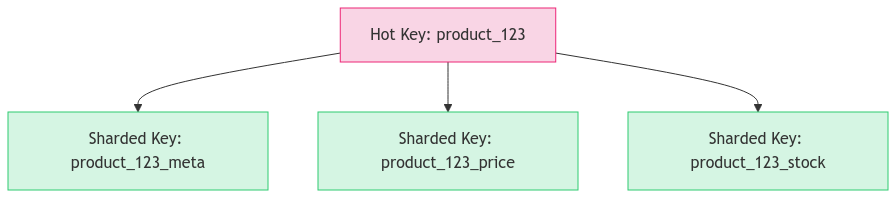
\includegraphics[width=0.9\textwidth]{images/sharding-hotkey.png}
		\caption{Contoh Sharding Hot Key \texttt{product\_123}}
		\label{fig:sharding-hotkey}
	\end{figure}
	
	\section{Manajemen TTL \& Invalidation}
	\label{sec:ttl-invalidation}
	
	\subsection{Atur TTL Dinamis}
	\label{subsec:ttl-dinamis}
	
	\begin{itemize}
		\item \textbf{Berdasarkan Pola Akses}:  
		\begin{itemize}
			\item Data yang sering diakses: TTL lebih panjang (misal: 1 jam).  
			\item Data jarang diakses: TTL lebih pendek (misal: 5 menit).  
		\end{itemize}
		
		\item \textbf{Berdasarkan Konteks Bisnis}:  
		\begin{itemize}
			\item Harga produk: TTL 1 menit (untuk update real-time).  
			\item Konten statis: TTL 24 jam.  
		\end{itemize}
		
		\item \textbf{Implementasi Dinamis}:  
		Gunakan algoritma adaptif seperti:  
		\[
		\mathrm{TTL} = \mathrm{Base\_TTL} + (\mathrm{Hit\_Rate} \times \mathrm{Adjustment\_Factor})
		\]
		Contoh: Jika hit rate 90\%, TTL = 5 menit + (0.9 × 10 menit) = 14 menit.
	\end{itemize}
	
	\subsection{Strategi Invalidation}
	\label{subsec:strategi-invalidation}
	
	\begin{itemize}
		\item \textbf{Event-Driven Invalidation}:  
		\begin{itemize}
			\item Picu invalidasi cache saat ada perubahan di database (gunakan CDC tools seperti Debezium).  
			\item Contoh: Saat harga produk di-update, kirim event ke sistem cache untuk menghapus \texttt{product\_<id>\_price}.  
		\end{itemize}
		
		\item \textbf{Write-Through Cache}:  
		\begin{itemize}
			\item Setiap operasi tulis ke database langsung memperbarui cache.  
			\item Cocok untuk data kritis seperti stok barang.  
		\end{itemize}
		
		\item \textbf{Timeout-Based Invalidation}:  
		\begin{itemize}
			\item Gunakan TTL singkat untuk data yang sering berubah (misal: 10 detik).  
		\end{itemize}
	\end{itemize}
	
	\begin{figure}[htbp]
		\centering
		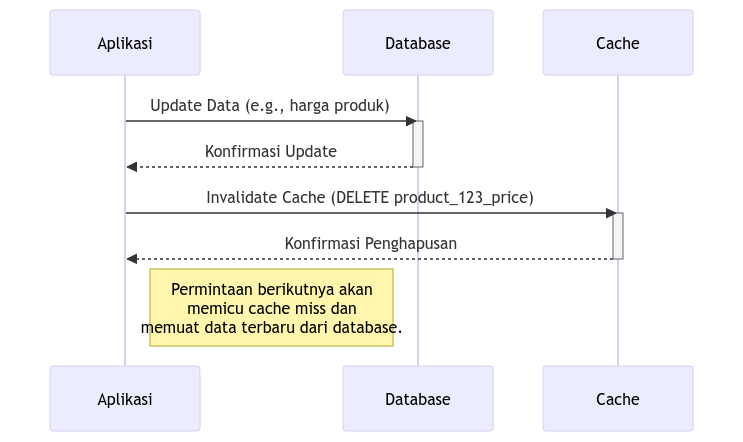
\includegraphics[width=0.9\textwidth]{images/cache-invalidation-sequence.png}
		\caption{Alur Event-Driven Cache Invalidation}
		\label{fig:invalidation-flow}
	\end{figure}
	
	\section{Monitoring \& Observability}
	\label{sec:monitoring}
	
	\begin{itemize}
		\item \textbf{Metric Kunci}:  
		\begin{itemize}
			\item \textbf{Hit Ratio}:  
			Rasio cache hit vs total request. Target: $>90\%$.  
			\[
			\mathrm{Hit Ratio} = \frac{\mathrm{Cache Hit}}{\mathrm{Cache Hit} + \mathrm{Cache Miss}}
			\]
			
			\item \textbf{Latensi}:  
			\begin{itemize}
				\item P95 latensi akses cache harus $<10$ ms.  
				\item Gunakan histogram untuk analisis distribusi.  
			\end{itemize}
			
			\item \textbf{Memory Usage}:  
			Pantau penggunaan memori per node. Hindari $>80\%$ kapasitas.  
		\end{itemize}
		
		\item \textbf{Tools Rekomendasi}:  
		\begin{itemize}
			\item Prometheus + Grafana untuk monitoring real-time.  
			\item Contoh Dashboard Grafana:  
			\begin{itemize}
				\item Panel hit ratio per service.  
				\item Heatmap latensi cache.  
				\item Alert saat memory usage $>75\%$.  
			\end{itemize}
		\end{itemize}
	\end{itemize}
	
	\begin{listing}[H]
		\begin{minted}[
			frame=lines,
			framesep=2mm,
			baselinestretch=1.2,
			bgcolor=LightGray,
			linenos,
			breaklines,
			]{yaml}
scrape_configs:
  - job_name: 'redis'
    static_configs:
      - targets: ['redis-node1:9121', 'redis-node2:9121']
    metrics_path: /scrape
    relabel_configs:
      - source_labels: [__address__]
        target_label: instance
		\end{minted}
		\caption{Contoh Konfigurasi Prometheus untuk Redis}	
	\end{listing}
	
	
	\section{Peringatan Penting}
	\label{sec:peringatan}
	
	\begin{itemize}
		\item \textbf{Cache Warming (Pemanasan Cache)}:  
		\begin{itemize}
			\item \textbf{Apa itu?}:  
			Proses memuat data ke cache sebelum permintaan aktual terjadi, biasanya saat startup aplikasi atau sebelum event traffic tinggi.
			
			\item \textbf{Mengapa penting?}:  
			Menghindari cache miss massal yang menyebabkan lonjakan beban database.
			
			\item \textbf{Cara Implementasi}:
			\begin{itemize}
				\item Jalankan script inisialisasi yang mengakses endpoint kritis saat aplikasi mulai.
				\item Contoh:  
				\begin{lstlisting}[language=bash,caption=Contoh Script Cache Warming]
# Panggil API produk populer saat startup
curl https://api.example.com/products/top-100
            \end{lstlisting}
			\end{itemize}
		\end{itemize}
		
		\item \textbf{Cache Stampede}:  
		\begin{itemize}
			\item \textbf{Apa itu?}:  
			Fenomena di mana banyak request bersamaan mencoba mengisi ulang cache yang sama saat data expired, menyebabkan overload pada database.
			
			\item \textbf{Contoh Kasus}:  
			1000 request/detik untuk data produk yang TTL-nya habis bersamaan.
			
			\item \textbf{Solusi}:
			\begin{itemize}
				\item \textbf{Probabilistic Early Expiration}:  
				Refresh cache secara acak sebelum TTL habis. Contoh:  
				\[
				\mathrm{TTL\_aktual} = \mathrm{TTL} - \mathrm{random}(0, \mathrm{TTL}/4)
				\]
				
				\item \textbf{Locking Mechanism}:  
				Gunakan distributed lock (e.g., Redis Redlock) untuk memastikan hanya satu request yang mengisi cache.
				
				\item \textbf{Contoh Kode}:
				\begin{listing}[H]
				\begin{minted}[
					frame=lines,
					framesep=2mm,
					baselinestretch=1.2,
					bgcolor=LightGray,
					linenos,
					breaklines,
					]{python}
def get_data(key):
    data = cache.get(key)
    if not data:
        if acquire_lock(key):
            try:
                data = db.query_data(key)
                cache.set(key, data, ttl=300)
            finally:
                release_lock(key)
    return data
				\end{minted}
				\caption{Penanganan Cache Stampede dengan Lock}	
				\end{listing}
				
			\end{itemize}
		\end{itemize}
	\end{itemize}
	
	\begin{table}[htbp]
		\centering
		\caption{Kapan Harus dan Tidak Harus Menggunakan Cache}
		\label{tab:cache-decision}
		\begin{tabularx}{\textwidth}{|l|X|X|}
			\hline
			\textbf{Kondisi} & \textbf{Cache} & \textbf{Jangan Cache} \\ \hline
			Frekuensi Akses & Tinggi ($>$100x/jam) & Rendah ($<$10x/jam) \\ \hline
			Ukuran Data & Kecil ($<$1 MB) & Besar ($>$10 MB) \\ \hline
			Volatilitas Data & Rendah (jarang berubah) & Tinggi (sering berubah) \\ \hline
			Contoh & Halaman beranda, session user & Laporan PDF, data audit \\ \hline
		\end{tabularx}
	\end{table}
	
	\chapter{Rangkuman \& Rekomendasi}
	\label{chap:rangkuman}
	
	\section{Poin Kunci}
	\label{sec:poin-kunci}
	
	\begin{itemize}
		\item \textbf{Distributed Caching Penting Untuk}:  
		\begin{itemize}
			\item Aplikasi dengan \textit{high traffic} dan kebutuhan responsivitas tinggi.
			\item Sistem yang memerlukan skalabilitas global dan toleransi kegagalan.
			\item Mengurangi biaya operasional dengan menurunkan beban database.
		\end{itemize}
		
		\item \textbf{Pemilihan Teknologi}:  
		\begin{table}[htbp]
			\centering
			\caption{Pedoman Pemilihan Teknologi Caching}
			\label{tab:pemilihan-teknologi}
			\begin{tabularx}{\textwidth}{|l|X|}
				\hline
				\textbf{Kebutuhan} & \textbf{Rekomendasi Tool} \\ \hline
				Kompatibilitas Redis + Open Source & Valkey \\ \hline
				Throughput ekstrem + multi-threaded & DragonflyDB \\ \hline
				Enterprise + komputasi terdistribusi & Hazelcast/Apache Ignite \\ \hline
				Sederhana + caching objek kecil & Memcached \\ \hline
			\end{tabularx}
		\end{table}
	\end{itemize}
	
	\section{Resource Lanjutan}
	\label{sec:resource}
	
	\subsection{Dokumentasi Resmi}
	\label{subsec:dokumentasi}
	
	\begin{itemize}
		\item \textbf{DragonflyDB}:  
		\href{https://dragonflydb.io/docs}{https://dragonflydb.io/docs} (Benchmark, konfigurasi klaster).
		
		\item \textbf{Redis}:  
		\href{https://redis.io/docs}{https://redis.io/docs} (Panduan struktur data, Redis Stack).
		
		\item \textbf{Valkey}:  
		\href{https://valkey.io/docs}{https://valkey.io/docs} (Migrasi dari Redis, best practices).
		
		\item \textbf{Memcached}:  
		\href{https://memcached.org/documentation}{https://memcached.org/documentation} (Optimasi memori).
		
		\item \textbf{Hazelcast}:  
		\href{https://docs.hazelcast.com}{https://docs.hazelcast.com} (Arsitektur enterprise).
	\end{itemize}
	
	\subsection{Pembelajaran Lanjut}
	\label{subsec:pembelajaran}
	
	\begin{itemize}
		\item \textbf{Redis University}:  
		\href{https://university.redis.com}{https://university.redis.com} (Gratis - kursus "Redis for Java Developers").
		
		\item \textbf{Buku Direkomendasikan}:  
		\begin{itemize}
			\item \textit{"Designing Data-Intensive Applications"} oleh Martin Kleppmann.
			\item \textit{"Redis in Action"} oleh Josiah Carlson.
		\end{itemize}
		
		\item \textbf{Video Tutorial}:  
		\begin{itemize}
			\item \href{https://www.youtube.com/watch?v=iuqZvajTOyA}{YouTube: System Design Interview - Distributed Cache} (34 menit).
		\end{itemize}
	\end{itemize}
	
	\section*{Aksi Selanjutnya}
	\label{sec:aksi}
	
	\begin{itemize}
		\item \textbf{Untuk Startup}:  
		Mulai dengan Redis/Memcached + pantau hit ratio. Migrasi ke DragonflyDB jika mencapai 10k RPM+.
		
		\item \textbf{Untuk Enterprise}:  
		Evaluasi Hazelcast/Apache Ignite untuk integrasi dengan sistem legacy.
		
		\item \textbf{Eksperimen Mandiri}:  
		\begin{itemize}
			\item Bandingkan latensi Redis vs DragonflyDB menggunakan \texttt{redis-benchmark}.
			\item Implementasi cache warming di aplikasi Anda.
		\end{itemize}
	\end{itemize}
	
	\begin{quote}
		\textit{"Caching is like salt - the right amount enhances performance, but too much ruins the system."} \\
		- Analogi Arsitek Sistem
	\end{quote}
	
\end{document}